\chapter{Epidemic Modelling}
\label{ch:progress}

\section{Motivations}
Modelling, is a technique commonly used in order to approximate an environment/system to gain insights and better understand possible outcome scenarios especially in situations when we don't have data available about the topic. Some examples of applications in which modelling is commonly applied are: climate change, military defense, designing cities, infecting diseases development and testing financial policies. 

Using modelling simulations, can be of great help when trying to answer different types of causal questions about our research topic (e.g. varying the different simulation parameters, it can be possible to see how these are related each other and how they effect the overall outcome). 

As part of this study, an interactive online Web Application \footnote{Web Application Link: \url{http://3.22.240.181:8501/}} has been developed in order to quickly analyse in real time COVID-19 developments and simulating different scenarios and approaches which can be taken in order to mitigate the consequences of this outbreak. Most of the provided models have been designed so that to be flexible enough to model any other type of possible future infectious disease. 

Additionally, a secondary website has been created using GitHub Pages in order to share additional notebooks and animations in Python and Julia \footnote{GitHub Pages Website Link: \url{https://pierpaolo28.github.io/Epidemics-Modelling/}}. 

\section{Introduction to Epidemiology}

\subsection{Different Classes of Diseases}
Infectious diseases, can mainly be classified into three different categories depending on their characteristics \cite{2minclass}:
\begin{enumerate}
    \item \textbf{Endemic}: an endemic is an health concern which is constantly present at a low rate within a population (its presence doesn't either substantially increase or decline). Some examples of endemics are Malaria and Chicken Pox.
    \item \textbf{Epidemic}: is an health issue which can cause a fast and unforeseen increase in cases within a population. An example of epidemic, can be considered the seasonal flu, which can lead to a sharp increase in the number of infected at specific times of the year.
    \item \textbf{Pandemic}: epidemics can finally later become pandemics if they manage to spread around the world and effect a great number of people. Some examples of pandemics are the Spanish Flu and COVID-19.
\end{enumerate}

\subsection{Exponential vs Logistic Growth}
\label{explog}
Pandemics, usually develops thanks to a disease ability to spread at an exponential rate. In the case of COVID-19, the number of cases from one day to the next was in fact equal to the number of nowadays cases times some constant between 1.25-1.5 (depending on factors such as population density and restrictions in place). The change in the number of cases from a day to another, can then be defined by the following equation \cite{exponentials}:

\useshortskip
\begin{align}
\ \Delta N_{d} = E \times p \times N_{d}
\label{n_new}
\end{align}
\useshortskip

Where $E$ represents the average number of people we are exposed to every day, $p$ represents the probability that an exposure might lead to an infection and $N_{d}$ is the number of cases as of today. Therefore, in this type of situation, the only possible way to try to slow down our exponential trend is by decreasing $E$ and $p$. In order to make this possible, different techniques such as track and trace, social distancing and travel restrictions can be applied. Although, even if no intervention at all is done, an exponential trend is destined to convert to a logistic curve once a large number of the population gets infected by the disease (in fact, the probability than an exposure can lead to an infect automatically decreases if the majority of the population and the people we meet are already infected). Applying any type of restriction, would then help us in making possible to reach our inflection point between these two trends as soon as possible.

Exponential growths, can be easier to inspect if when plotting them on a logarithmic scale. Using this type of graph, an exponential curve would then look like approximately a straight line. As we can see from the graph on the left of Figure \ref{exp}, all the different considered countries follow the at first the same exponential pattern which then seems to be starting converting to a logistic curve. The graph on the right of Figure \ref{exp}, was then designed in order to try to amplify this change \cite{physics}. While going through an exponential growth, it can be difficult to understand how long will it last (if the growth is going to still keep being exponential or is going to start decaying). One possible way to approach this problem, is to focus our attention on the rate of change in new cases from a week to another. Plotting this on a both axis logarithmic scale, we would then clearly see that all the different countries have a same linear growth in cases. Although, using some form of containment, some of these countries are successfully able to escape from this linear growth in cases. Using this type of approach, we can successfully emphasize the deviation in the growth of an exponential curve.

\begin{figure}[ht!]%
    \centering
    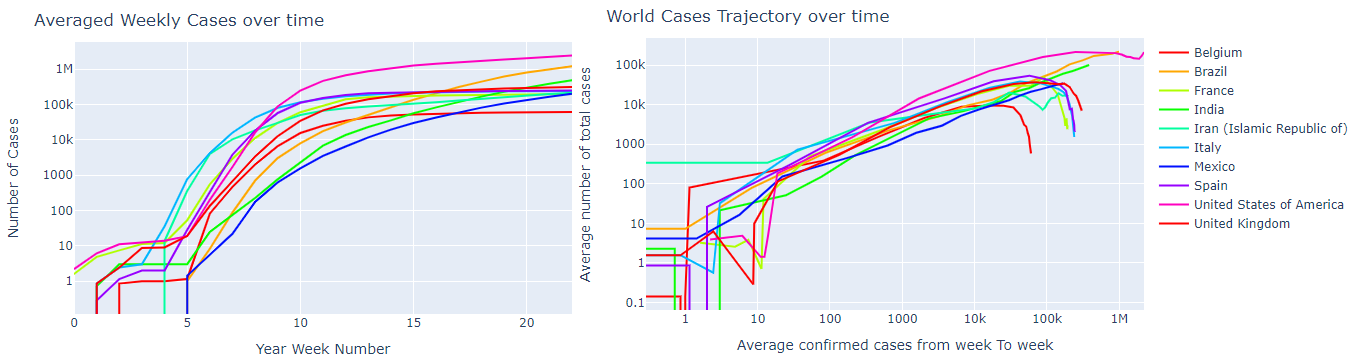
\includegraphics[width=17cm]{latex/images/logplot.png}%
    \caption{Exponential Growth Evolution}
    \label{exp}
\end{figure}

Using the logarithmic linear graphs, we could then perform a linear regression to find the line of best fit and find out how many days does it take for our cases to increase by a fixed constant. Finally, using metrics such as the $R^{2}$ score, we could then quantitatively measure how far are our curves from an exponential curve.

Another way to examine if we are reaching the end of an exponential curve, is by examining the slope (Growth Factor, Equation \ref{growth}).

\useshortskip
\begin{align}
\ Growth \; Factor = \dfrac{\Delta N_{d}}{\Delta N_{d-1}}
\label{growth}
\end{align}
\useshortskip

A growth factor of more than one, will show us that we are still going through an exponential growth, while a growth factor equal to 1 can tell us we might now be approaching our inflection point.

A worked out example of logistic/exponential curve fitting on real world Coronavirus data, is Available in Appendix \ref{exp_fit}.

\subsection{Quantifying the spread of a disease}
One of the main unit used to measure how easily a disease is able to diffuse in a community is the "Effective Reproductive Number" ($R$), which is measured as the average number of people infected by each individual carrying the disease. In a fully susceptible population, $R$ is also referred as $R_{0}$ ("Basic reproductive Number"). The Basic reproductive Number for COVID-19 is currently estimated to be around 2.5.

As shown in Equation \ref{r0}, $R_{0}$ can be calculated as the number of people someone positive to the disease can infect each day ($\beta$) multiplied by the number of days each person remains positive to the disease ($D$). Equivalently, $R_{0}$ can also be estimated as the number of people someone positive to the disease can infect each day multiplied by the proportion of individuals infected recovering each day ($\gamma = 1/D$). Furthermore, as shown in Equation \ref{day_inf}, $\beta$ can be also calculated to be equal to the probability that an exposure might lead to an infection ($p$) multiplied by the average number of people we are exposed to every day ($E$) \cite{tds}.

\useshortskip
\begin{align}
\ R_{0} = \beta \times D = \dfrac{\beta}{\gamma}
\label{r0}
\end{align}
\useshortskip

\useshortskip
\begin{align}
\ \beta = E \times p
\label{day_inf}
\end{align}
\useshortskip

If $R$ is greater than one, then the disease is still in the exponentially growing phase (we have an epidemic), if $R$ is instead equal to one we are instead in an endemic (therefore the number of cases stays approximately constant) and if $R$ is less than one, we are instead in the eradication phase and the disease could disappear entirely soon from our population.

One of the most common approaches to eradicate a decease, is through Herd Immunity. The percentage proportion of the individuals in a population necessary to reach Herd Immunity can be estimated using Equation \ref{immunity}. In the case of COVID-19, this is estimated to be around 60\%. Herd Immunity, can potentially be achieved either through vaccination or natural selection \cite{blob}.

\useshortskip
\begin{align}
\ Herd\:Immunity\:(H.I.) = 1 - \frac{1}{R_{0}}
\label{immunity}
\end{align}
\useshortskip

Different typology's of Epidemics Modelling have been developed in the past few years, such as:
\begin{itemize}
    \setlength\itemsep{-0.3cm}
    \item Compartmental Models
    \item Agent Based Models
    \item Network Models
    \item Meta-populations Models
\end{itemize}

In this chapter, we will explore the first two approaches.

\section{Compartmental Models}

In Compartmental Models, is assumed that each individual in a population, is assigned to a compartment. During the course of the simulations, individuals can then be free to move from one compartment to another depending on the dynamics of the model. Some examples of common departments in Epidemic Modelling are: Susceptible, Exposed, Infectious, Recovered, Dead, Vaccinated, etc...

This models can be designed using either ordinary differential equations or stochastic elements as well. Diagrams representations of this type of models can be of great help in order to understand how the model equations works and what are the possible movements between different states. 

\subsection{SIR (Susceptible-Infected-Recovered)}

\textbf{Causal Question:} How does the number of people I am in contact with on average in a day affect the evolution of the pandemic?

\textbf{Experimental Results:} The SIR model is one of the most widely used epidemiology model and is composed by just 3 different compartments: Susceptible ($S$), Infected ($I$) and Recovered ($R$). This model can be described by the following three formulas, where 
$N$ is the total number of elements in the population, $\beta$ represents average amount of people an infected element can be able to infect in a day and
$\gamma$ the percentage of how many individuals recover from the disease each day.

\useshortskip
\begin{align}
\ \frac{\partial S}{\partial t} = -\beta \times I \times \frac{S}{N}
\end{align}
\useshortskip

\useshortskip
\begin{align}
\ \frac{\partial I}{\partial t} = \beta \times I \times \frac{S}{N} -\gamma \times I
\end{align}
\useshortskip

\useshortskip
\begin{align}
\ \frac{\partial R}{\partial t} = \gamma \times I
\end{align}
\useshortskip

In order to visualise better the situation, this set of equations, can then be converted into a block diagram representation using the following structure (Figure \ref{comp}).

\begin{figure}[ht!]%
    \centering
    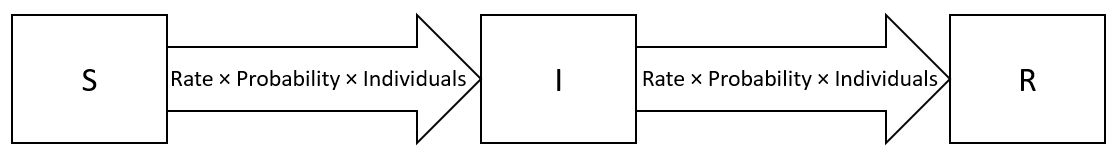
\includegraphics[width=13cm]{latex/images/comp.PNG}%
    \caption{Compartmental Models Diagram Representation}
    \label{comp}
\end{figure}

Therefore, in order to move from one compartment to another, we need to take into consideration how long would this transaction take (Rate), the probability that it will actual happen for each individual (Probability) and the portion of individuals for which this transition takes place (Individuals). Converting our SIR set of equations into this representation, we can then obtain the diagram in Figure \ref{dsir}. When converting between these two representations, we can then see how a minus sign in the Ordinary Differential Equation (ODE) corresponds to an arrow leaving that compartment, while a plus sign corresponds to an arrow pointing towards that compartment. This same procedure can then be used in order to design any other type of compartmental model.

\begin{figure}[ht!]%
    \centering
    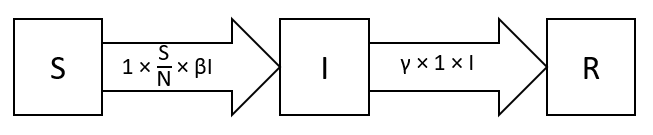
\includegraphics[width=10cm]{latex/images/dsir.PNG}%
    \caption{SIR Diagram Representation}
    \label{dsir}
\end{figure}

Using the parameters in Table \ref{table:1}, it can then be possible to obtain the results in Figure \ref{sir}.

{
\begin{table}[h!]
\centering
\begin{tabular}{|c|c|}
\hline
Parameter Type & Value \\
\hline
Population Size & 100  \\
Number of Days & 100  \\
Number of individuals originally infected & 3  \\
Number of individuals at close contact in a day & 5 \\
Probability of infection if in contact with an infected & 0.1\% \\
Number of days a the disease can last & 7 \\
\hline
\end{tabular}
\caption{SIR Model Parameters}
\label{table:1}
\end{table}
}


\begin{figure}[ht!]%
    \centering
    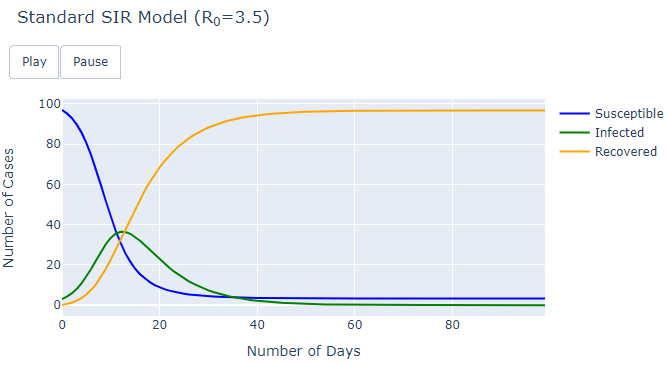
\includegraphics[width=13cm]{latex/images/sir.PNG}%
    \caption{SIR Model}
    \label{sir}
\end{figure}

\subsection{SEIR (Susceptible-Exposed-Infected-Recovered)}

In order to make our more more realistic, we can then add an additional state E representing all the population elements which are still in the incubation stage before becoming infected. In order to apply these modifications, we just need to update $\frac{\partial I}{\partial t}$ and add this extra stage before just before it. The only variable which needs to be added compared to the SIR model is the proportion of how many individuals move from the incubation period to being infected ($\delta = \dfrac{1}{Days\;of\;incubation}$).

\useshortskip
\begin{align}
\ \frac{\partial E}{\partial t} = \beta \times I \times \frac{S}{N} -\delta \times E
\end{align}
\useshortskip

\useshortskip
\begin{align}
\ \frac{\partial I}{\partial t} = \delta \times E \times -\gamma \times I
\end{align}
\useshortskip

Following the same procedure as for the SIR model, we can then convert our SEIR model in block diagram form (Figure \ref{dseir}).

\begin{figure}[ht!]%
    \centering
    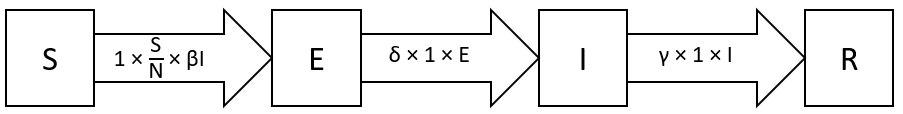
\includegraphics[width=10cm]{latex/images/dseir.PNG}%
    \caption{SEIR Diagram Representation}
    \label{dseir}
\end{figure}

Using the same parameters as in Table \ref{table:1}, and using one day as the number of incubation days for the disease, can then be produced the results in Figure \ref{seir}.

\begin{figure}[ht!]%
    \centering
    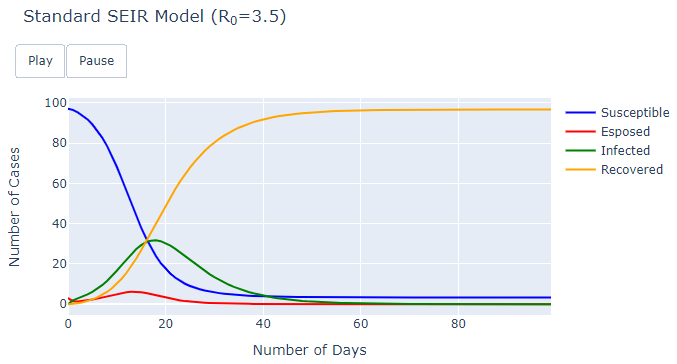
\includegraphics[width=13cm]{latex/images/seir.PNG}%
    \caption{SEIR Modelling}
    \label{seir}
\end{figure}

\subsection{Advanced SEIR Modelling}
\label{cov_model}

\textbf{Causal Question:} What are the effects of varying social distancing measures over time using different approaches (landscapes)? Given some user defined population age distribution, how would that effect the overall number of deaths?

\textbf{Experimental Results:} Starting from the developed SEIR Model, it can be now possible add more compartments and make different elements time-dependent so that to better capture real-world dynamics. The main additions engineered in this model are:
\begin{itemize}
    \item Take into account the portion of infected individuals which dies instead of recover. This can be done by adding a new compartment after the Infected Stage and introducing two new variables $\rho$ (the rate, in terms of days, which takes on average to die) and $\alpha$ (the disease death rate) which determines the probability an individual infected might either die or recover.
    \item $R_{0}$ is not anymore static but dynamically changes over time. In this example, two functions have been used  in order to simulate $R_{0}$ behaviour over time: a Sigmoid or Sinusoidal. In this way, we are now able to model
    how a government might react in order to control the spread of the disease by exercising social distancing measures. A sigmoid in it's minimum point can in fact represent a lock-down and the smoothness by which it reaches its minimum can
    easily represent how gradually the restrictions have been applied. An additional parameter is provided in order to decide from what day onward to start applying the restrictions (so that to observe what could be the consequences of a late or early intervention). The sinusoidal landscape, can instead be used in order to model possible sequential waves a disease can lead to. Because, $\beta$ is dependent on  $R_{0}$, this will be indicated to be our time dependent variable in our set of ODEs. 
    \item Also the death rate has been designed to be time and age dependent. To each different age group is assigned a different base death rate (the older, the greater), which increase linearly with the increase in the number of infected at each time-step. Therefore, with higher peaks of individuals infected all at the same time increases the likelihood of individuals to die (mimicking strained healthcare system which don't have the potential to cure everyone at the same time).
\end{itemize}

The main equations summarising the flow between the different compartments can be summarised as:

\useshortskip
\begin{align}
\ \frac{\partial S}{\partial t} = -\beta(t) \times I \times \frac{S}{N}
\end{align}
\useshortskip

\useshortskip
\begin{align}
\ \frac{\partial E}{\partial t} = \beta(t) \times I \times \frac{S}{N} -\delta \times E
\end{align}
\useshortskip

\useshortskip
\begin{align}
\ \frac{\partial I}{\partial t} = \delta \times E - (1 - \alpha(t)) \times \gamma \times I - \alpha(t) \times \rho \times I
\end{align}
\useshortskip

\useshortskip
\begin{align}
\ \frac{\partial R}{\partial t} = (1 - \alpha(t)) \times \gamma \times I
\end{align}
\useshortskip

\useshortskip
\begin{align}
\ \frac{\partial D}{\partial t} = \alpha(t) \times \rho \times I
\end{align}
\useshortskip

Which results in the following diagram flow architecture:

\begin{figure}[ht!]%
    \centering
    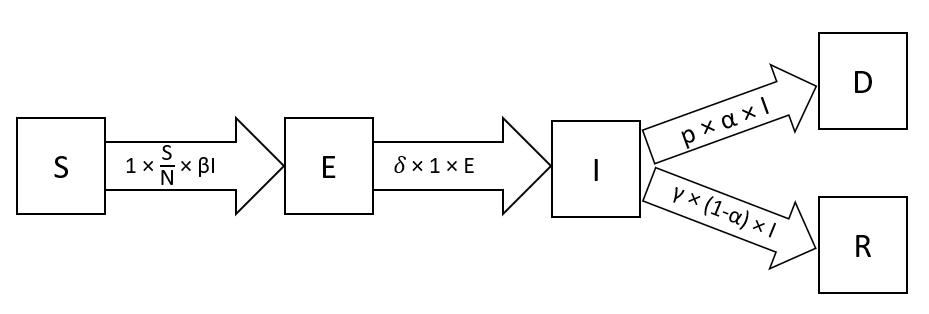
\includegraphics[width=10cm]{latex/images/dadv_seir.PNG}%
    \caption{Advanced SEIR Diagram Representation}
\end{figure}

More specifically, the adaptive $R_{0}$ for the Sigmoid case has been designed to be equal to Equation \ref{sig}.

\useshortskip
\begin{align}
\ R_{0}(t) = \frac{R_{start}-R_{end}}{1 + \exp^{-k(-x+x_{0})}} - R_{end}
\label{sig}
\end{align}
\vspace{-0.4cm}
\begin{conditions}
 $R_{start}, R_{end}$  &  Initial and desired final value for $R_{0}$ in the sigmoid \\
 $x_{0}$  &  Sigmoid inflection point date\\
 $k$  &  Defines how drastically rapidly the restrictions have been applied\\
\end{conditions}
\vspace{-0.2cm}
\useshortskip

Following from our $R_{0}(t)$ calculation, $\beta(t)$ can then be estimated to be equal to:
\useshortskip
\begin{align}
\ \beta(t) = R_{0}(t) \times \frac{1}{\alpha \times \frac{1}{\rho} + (1 - \alpha) \times \frac{1}{\gamma}}
\end{align}
\useshortskip

In the case of a Sinusoidal landscape, $R_{0}$ has instead designed to be dependent on the following expression:

\useshortskip
\begin{align}
\ R_{0}(t) = Oscillatory\:Scale \times \sin(\frac{x}{\frac{N\:Simulation\:Days}{10}}) + Oscillatory\:Scale + 1
\end{align}
\useshortskip

In this way, $R_{0}$ is designed to always go through two peaks and one low for any type of possible simulation. Using an $Oscillatory\:Scale$ of 1, the peaks will be equal to an $R$ value of 3, while the low would be equal to 1. Increasing the value of the $Oscillatory\:Scale$, will then lead to higher values for our landscape peaks.

Finally, in order to make our death rate time variant and dependent on the population age and number of infected cases at the same time, the following expression has been used:

\useshortskip
\begin{align}
\ \alpha(t) = s \times \frac{I(t)}{N} + \alpha_{opt}
\end{align}
\vspace{-0.4cm}
\begin{conditions}
 $s$  &  Regulates in what proportion the death rate rises when 
 the number of \\ 
 & infected increases. \\
 $\alpha_{opt}$  &  The death rate calculated depending on the population age.  \\ & Overall older populations will therefore have an higher base death rate \\
 & than younger populations.\\
\end{conditions}
\vspace{-0.2cm}
\useshortskip

This advanced SEIR version has been inspired by Henri Froese \cite{tds} work.

Starting with the same parameters already specified for the SIR and standard SEIR model we can then specify the number of days the disease can take to become lethal to be equal to 3 and the percentage weight of age on the death rate to 30\%.

The proportions of individuals within different age ranges, could then be specified as shown in \ref{table:3}.

\vspace{-0.3cm}
{
\begin{table}[h!]
\centering
\begin{tabular}{|c|c|c|c|c|}
\hline
\multirow{2}{*}{Demographic} & \multicolumn{4}{c|}{Age} \\\cline{2-5}
& 0-20 & 20-50 & 50-70 & 70-110 \\
\hline
Proportion Percentage (\%) & 0.15 & 0.25 & 0.4 & 0.2 & 
\hline
\end{tabular}
\caption{Population Demographics}
\label{table:3}
\vspace{-0.4cm}
\end{table}
}

In the case of the Sigmoid Landscape, using the parameters in Table \ref{table:4}, has been possible to record the results in Figure \ref{sig_seir}.
{
\begin{table}[h!]
\centering
\begin{tabular}{|c|c|}
\hline
Parameter Type & Value \\
\hline
Social Distancing start date & 20  \\
Percentage weight of how rapidly the restrictions are applied & 30\%  \\
Maximum possible R value & 5  \\
Minimum possible R value & 1  \\
\hline
\end{tabular}
\caption{Sigmoid Landscape Parameters}
\label{table:4}
\end{table}
}

\begin{figure}[ht!]%
    \centering
    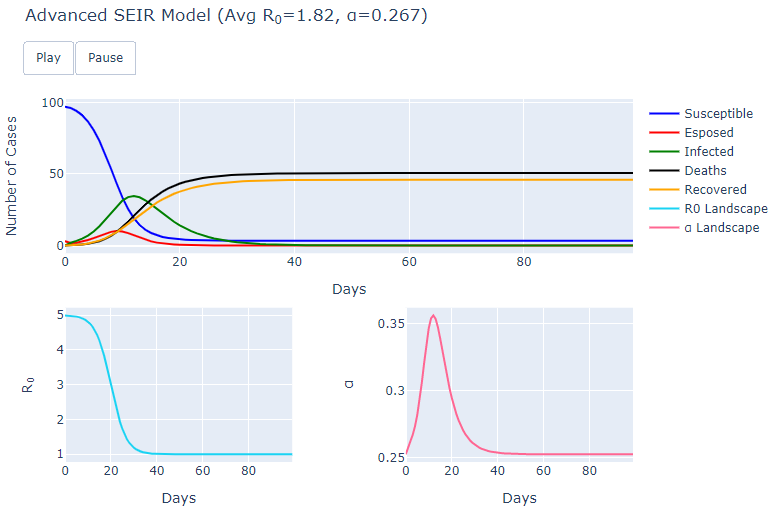
\includegraphics[width=13cm]{latex/images/sig_seir.PNG}%
    \caption{Advanced SEIR (Sigmoid) Modelling}
    \label{sig_seir}
\end{figure}

Using instead the Sinusoidal landscape and a scaling factor of 2, have been registered the results in Figure \ref{sine_seir}.

\begin{figure}[ht!]%
    \centering
    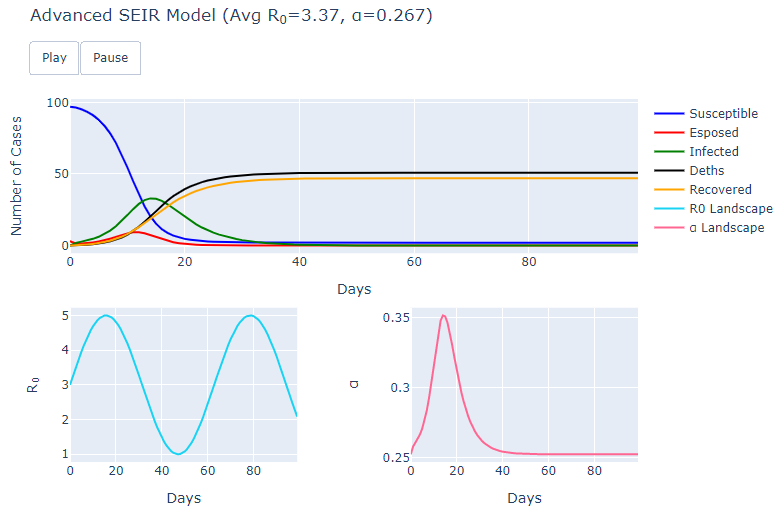
\includegraphics[width=13cm]{latex/images/sine_seir.PNG}%
    \caption{Advanced SEIR (Sinusoidal) Modelling}
    \label{sine_seir}
\end{figure}

\subsection{Time Limited Immunity and Vaccination Modelling}

\subsubsection{Time Limited Immunity}

Updating our SIR model, we can be able to take into account the possibility that individuals might not gain lifetime immunity from a disease when recovering from it, but that might instead be re-infected again in the future after some time. The amount of time an individual might be immune from a disease can be represented by just adding a new variable to our model ($v$) \cite{immune}.

\useshortskip
\begin{align}
\ \frac{\partial S}{\partial t} = -\beta \times I \times \frac{S}{N} + v \times R
\end{align}
\useshortskip

\useshortskip
\begin{align}
\ \frac{\partial I}{\partial t} = \beta \times I \times \frac{S}{N} -\gamma \times I
\end{align}
\useshortskip

\useshortskip
\begin{align}
\ \frac{\partial R}{\partial t} = \gamma \times I - v \times R
\end{align}
\useshortskip

Converting our set of equations into a Block Diagram representation, will then result in Figure \ref{dimm}.

\begin{figure}[ht!]%
    \centering
    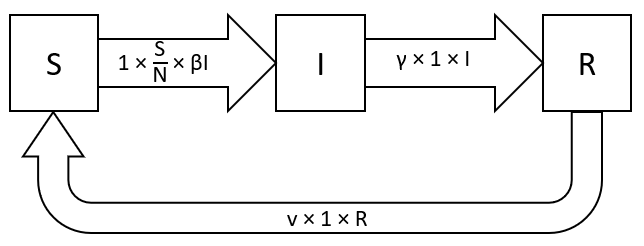
\includegraphics[width=10cm]{latex/images/dimm.PNG}%
    \caption{SIR Time Limited Immunity Diagram Representation}
    \label{dimm}
\end{figure}

Using the same SIR model parameters as in Table \ref{table:1}, setting to 25 the maximum number of days the immunity to the disease can last, we can then produce the following results in Figure \ref{low_imm}.

\begin{figure}[ht!]%
    \centering
    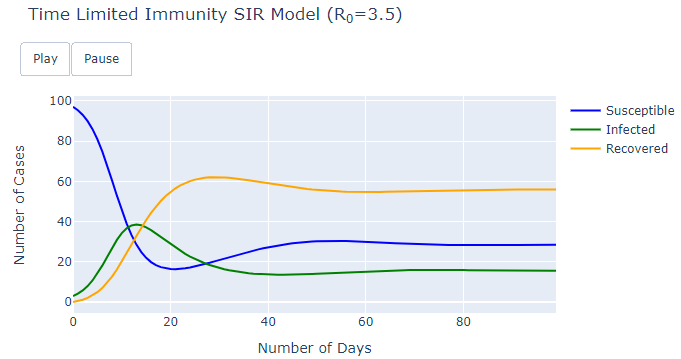
\includegraphics[width=13cm]{latex/images/time_lim.PNG}%
    \caption{Time Limited Immunity Modelling}
    \label{low_imm}
\end{figure}

\subsubsection{Vaccination}

Extending our set of equations (adding an extra stage $\frac{\partial V}{\partial t}$), we can be able to take into account how an epidemic will evolve once a vaccine is available. In order to apply these modifications, we just need to update $\frac{\partial S}{\partial t}$ and add the vaccination stage before just after it. To make the simulation more realistic, we can then also specify from when in time a vaccine could start being distributed and how fast it can produced and shipped ($p$). Finally, a stage used to record the possible amount of deaths is included (using the same notation for the Advanced SEIR models).

\useshortskip
\begin{align}
\ \frac{\partial S}{\partial t} = -\beta \times I \times \frac{S}{N} + v \times R - p \times S
\end{align}
\useshortskip

\useshortskip
\begin{align}
\ \frac{\partial V}{\partial t} = p \times S
\end{align}
\useshortskip

\useshortskip
\begin{align}
\ \frac{\partial I}{\partial t} = \beta \times I \times \frac{S}{N}  -(1-\alpha) \times \gamma \times I -\alpha \times \rho \times I
\end{align}
\useshortskip

\useshortskip
\begin{align}
\ \frac{\partial R}{\partial t} = (1-\alpha) \times \gamma \times I - v \times R
\end{align}
\useshortskip

\useshortskip
\begin{align}
\ \frac{\partial D}{\partial t} = \alpha \times \rho \times I
\end{align}
\useshortskip

Converting our set of equations into a Block Diagram representation, we can then obtain Figure \ref{dvacc}.

\begin{figure}[ht!]%
    \centering
    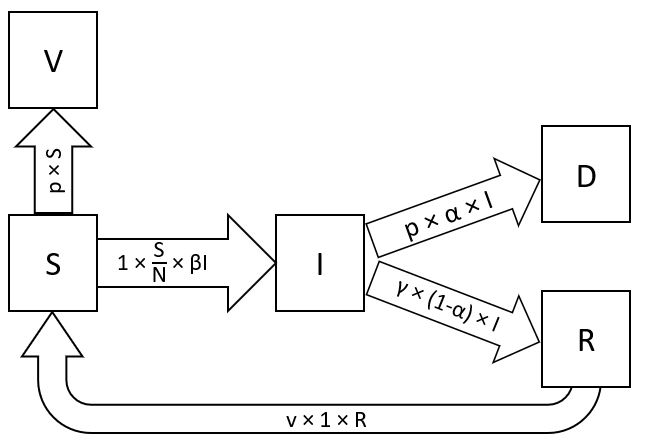
\includegraphics[width=10cm]{latex/images/dvacc.PNG}%
    \caption{SIR Time Limited Immunity and Vaccination Diagram Representation}
    \label{dvacc}
\end{figure}


Extending our set of parameters used for the Time Limited Immunity model, using the values from Table \ref{table:2}, has been possible to obtain the results in Figure \ref{vacc}.

{
\begin{table}[h!]
\centering
\begin{tabular}{|c|c|}
\hline
Parameter Type & Value \\
\hline
Number of days the disease can take to become lethal & 5  \\
Death rate & 0.2\%  \\
Number of Days to start Vaccine Distribution & 30  \\
Vaccine Distribution rate & 0.1\%  \\
\hline
\end{tabular}
\caption{SIR Vaccination Model Parameters}
\label{table:2}
\end{table}
}

\begin{figure}[ht!]%
    \centering
    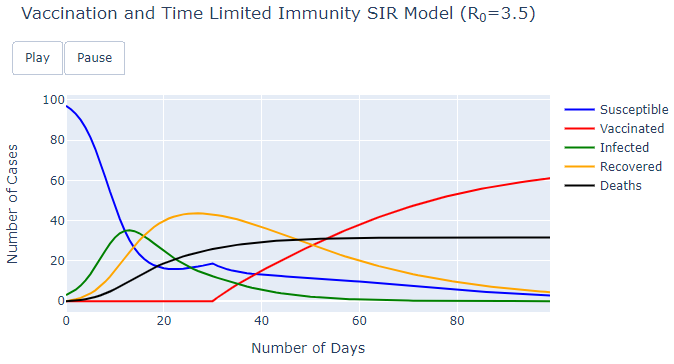
\includegraphics[width=13cm]{latex/images/vacc.PNG}%
    \caption{Vaccination Modelling}
    \label{vacc}
\end{figure}

Making use of the provided Time Limited Immunity and Vaccination models, in conjunction with Equation \ref{immunity}, it could then be possible to get estimates of what proportion of the population would be necessary in order to gain Herd Immunity. 

\subsection{Coronavirus Modelling}
In order to test on real world data one of the created models, the architecture of the Advanced SEIR model outlined in Section \ref{cov_model} has been tested. The different parameters of the model, have then been personalised depending on the examined country specifics.

In order to do so, information about a large number of countries population size and demographics has been processed making use of the United Nations World Population Prospects 2019 dataset \cite{pop_data}. Additionally, information about the number of hospital beds available for 1000 people for each country has been used from the The World Bank Data Hospital Beds dataset \cite{beds_data}, in order to calculate estimates of when hospitals in different countries might get overwhelmed and how many avoidable deaths would that cause.

Finally, an estimation of the number of actual cases for each country has been calculated using the approach outlined in "Substantial undocumented infection facilitates the rapid dissemination of novel coronavirus (SARS-CoV-2)" \cite{cases_paper}.

\subsubsection{Germany Case Study}

\textbf{Causal Question:} How can we prevent an healthcare system to become overwhelmed? How many lives would be saved?

\textbf{Experimental Results:} As of the 29th of June 2020, Germany Coronavirus record can be summarised as in Figure \ref{germ}. Germany has a total population of 84 millions and the total number of estimated cases has been calculated taking in consideration that about 86\% of the total Coronavirus cases have been estimated to have been undocumented \cite{cases_paper} in China.

\begin{figure}[ht!]%
    \centering
    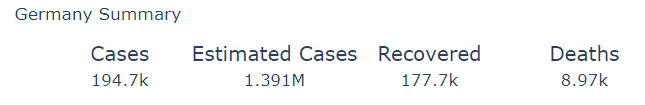
\includegraphics[width=12cm]{latex/images/cov_g.PNG}%
    \caption{Germany Statistics}
    \label{germ}
\end{figure}

Another point, which could be necessary to take into account in order to understand the true number of cases in a country is the possibility of false positives and false negatives during testing. More accurate estimates can be calculated using Bayes Rule and the Law of Total Probability (Equation \ref{bayes2}). For instance, is a patient does a Coronavirus test and results positive, what are its chances that he/she actually has Coronavirus?

\useshortskip
\begin{align}
\ P(B|A) = \frac{P(A|B)\times P(B)}{P(A)} = \frac{P(A|B)\times P(B)}{P(A|B)\times P(B) + P(A|\stcomp{B})\times P(\stcomp{B})}
\label{bayes2}
\end{align}
\useshortskip

In this example, we are going to take into consideration the COVID-19: Roche Antibody Test \cite{roche}. This test, has an estimated sensitivity of 100\% (ability to correctly identify patients with the disease) and specificity of 99.8\% (ability to correctly identify patients without the disease). Assuming a prevalence of the disease in the population of about 5\%, the following estimates can be calculated:

\useshortskip
\begin{align}
\ P(B|A) = \frac{1 \times 0.05}{1 \times 0.05 + 0.002 \times 0.95} = 96.33\%
\end{align}
\useshortskip

If the test is positive, there would be then a 96.33\% probability the patient actually has Coronavirus. As can be seen from Equation \ref{bayes2}, the rate of the Coronavirus cases in a population, plays an important factor.

An example of a simulation run, using Germany as case study is available below. As can be noticed, the key difference between \ref{germ_sim} and \ref{sig_seir} is the fact that we are to take into account this time also when the healthcare system of the selected country runs out of beds for critical patients. This can be of vital help, in order to understand to what limit the healthcare system can be able to provide support the all the patients in need at any point in the pandemic and how many deaths could be avoided.
 
\begin{figure}[ht!]%
    \centering
    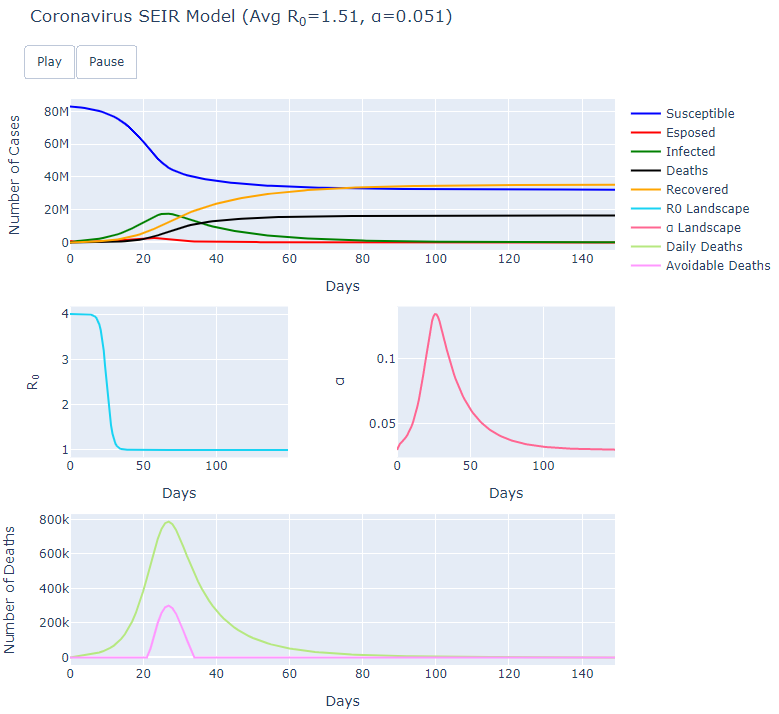
\includegraphics[width=13cm]{latex/images/cov_g2.PNG}%
    \caption{Germany Simulation}
    \label{germ_sim}
\end{figure}

Additionally, an estimate of the number of beds needed to go through the peak of the simulated pandemic while providing support for all the critically ill patients is provided in Figure \ref{germ_bed} alongside with the current number of beds available.

\begin{figure}[ht!]%
    \centering
    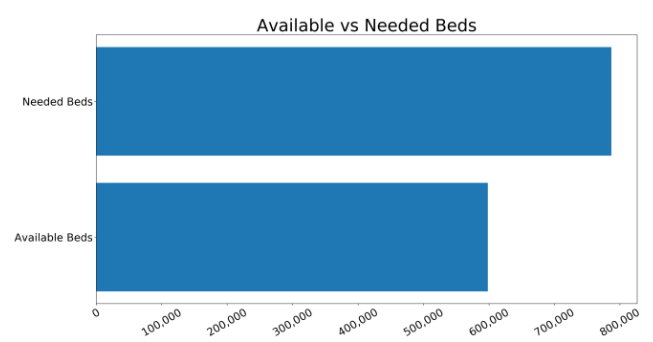
\includegraphics[width=9cm]{latex/images/cov_g3.PNG}%
    \caption{Germany Hospital Beds Analysis}
    \label{germ_bed}
\end{figure}

Finally, is calculated an automatic estimation of the parameters of the Advanced SEIR model given the provided data. This estimation is computed using non-linear least squares and the final $R^{2}$ score is provided as metric for the convergence of the fitted curve compared to the original one. According to these estimates, thanks to public health restrictions, Germany $R$ value, varies from a maximum of 6.37 to a minimum of 1.45 during the last 5 months.

\begin{figure}[ht!]%
    \centering
    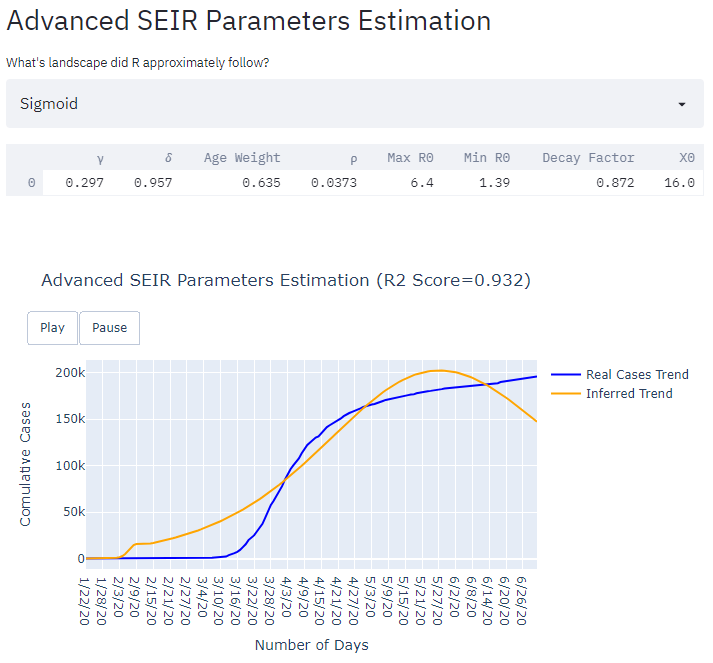
\includegraphics[width=13cm]{latex/images/germ_params.PNG}%
    \caption{Advanced SEIR Parameters Estimation}
\end{figure}

\section{Agent Based Models}
An alternative approach which can be used in order to simulate compartmental-like models, is by creating an Agent Based simulation. In this case, each single individual in the population is created following an Objected Oriented Programming approach (eg. using a programming class) and it's behaviour in an environment while in contact with the rest of the population is simulated. Using this type of approach, can therefore enable us to keep track of the position of the different individuals in a population and attribute then different characteristics such as an age or daily income. Similar results could be obtained using standard compartmental models by converting our Ordinary Differential Equations into Partial Differential Equations and making them dependent on both time and space \cite{pde}.

The proposed Agent Based Model, is directly inspired from The Epidemiological Triad paradigm (Figure \ref{triad}).

\begin{figure}[h]
\vspace{-0.2cm}
\centering
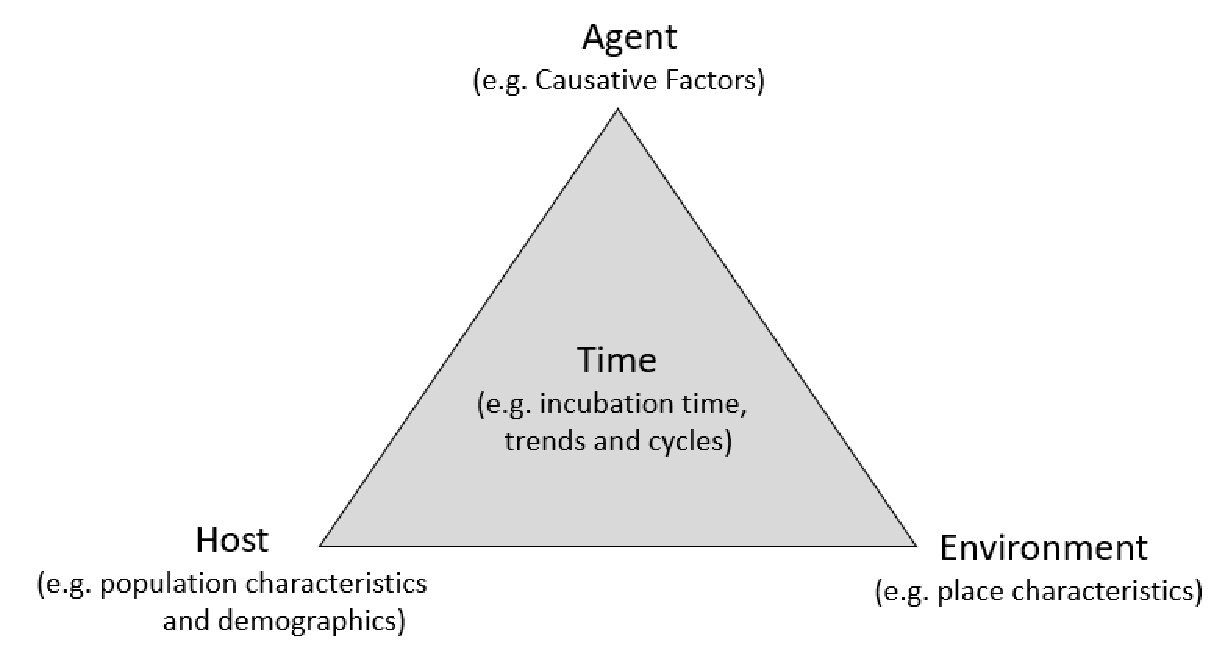
\includegraphics[scale = 0.5]{latex/images/model.pdf}
\caption{The Epidemiological Triad}
\label{triad}
\end{figure}

\subsection{Population Modelling}

\textbf{Causal Question:} How does population density and community distribution affect the spread of a disease?

\textbf{Experimental Results:} As described in Section \ref{explog}, the number of new cases can vary according to Equation \ref{n_new}. Therefore, the only way we can be able to decrease the number of cases, is by decreasing the values of $E$ and $p$. 
\begin{itemize}
    \setlength\itemsep{-0.3cm}
    \item $E$ can decrease if travelling and meetings of people are reduced as much as possible.
    \item $p$ can be reduced instead for example by making less likely to catch the disease by taking precautions such as washing hands, wearing masks, avoid touching our faces, etc...
\end{itemize}

This trend can be observed in the following proposed model (Algorithm \ref{alg1}) by the \textbf{Contact Radius} ($E$) and \textbf{Probability of how unlikely it is to spread the virus if within the contact radius} (complementary of $p$) variables.
In this way, causal effects of social distancing and improved hygiene can be easily inspected. Furthermore, the role of dividing individuals in different communities is additionally studied. Having different communities with a central shared point and random infected initialization, can in fact resemble how contagious disease hot-spots can be created.

An example output of this type of simulation, is available in Figure \ref{pop}.

\begin{figure}[ht!]%
    \centering
    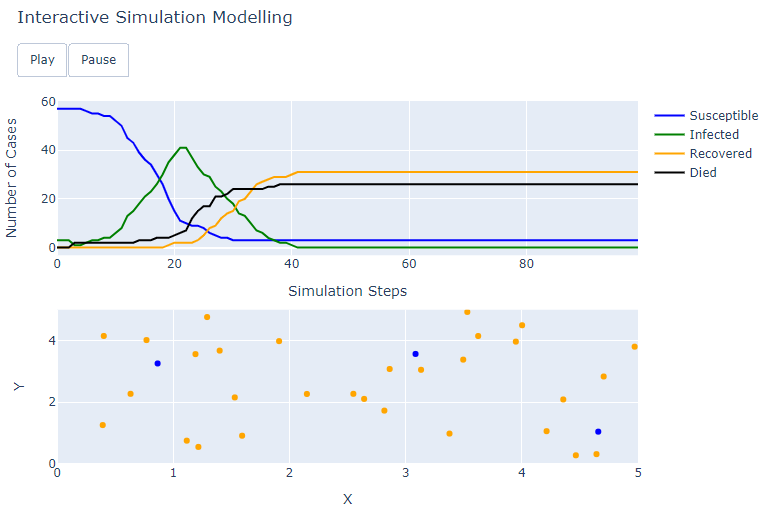
\includegraphics[width=13cm]{latex/images/pop.PNG}%
    \caption{Population Modelling}
    \label{pop}
\end{figure}

In this type of model, each of the individual is born with unique combination of characteristics such as: their situation (susceptible to the virus, positive, recovered or dead), position in X and Y coordinates on a grid which represents their world, the speed with which they move and the X and Y directions at which they point to (e.g. mimicking individuals commuting from one place to another every time), a counter used to keep track of how many days of rehabilitation an individual went through with the virus and the individual age (the greater the age, the more likely to die). 

An original death probability is assigned to each individual, indicating the probability someone would have to die for any general reason (this base probability is then increased depending on age if being affected by the virus). In this case, the death probability is defined as:

\useshortskip
\begin{align}
\ Updated\:Death\:Probability = Death\:Probability \times (\frac{Age}{100} + 1) 
\end{align}
\useshortskip

For example, if a 50 years old individual has a base probability to die of 1\%, this will be increased because of the virus to 1.5\%. Additionally, a Boolean value (\textbf{Static}) can be used in order to make the population static (therefore mimicking the effect of being permanently in a same location in order to avoid spreading the virus).

During each iteration, using the Euclidean Distance in Equation \ref{euc}, is measured how close each individual is with the others in the space and if it is close to some people affected by the virus (within the defined Contact Radius). The number of occurrences are then counted and the more they are and the more likely it will be that the individual will catch the virus (how likely it is that someone can catch the virus is additionally dependent on the specified probability of how unlikely is it to catch the virus - the lower it is and the more likely we will become infected).

\useshortskip
\begin{align}
\ d = \sqrt{(x_{2}-x_{1})^{2}+(y_{2}-y_{1})^{2}}
\label{euc}
\end{align}
\useshortskip

Additionally, each iteration is kept an eye on the individuals affected by the virus. Each iteration depending on the mortality probability different individuals might die and if an individual survives for 14 iterations without dying, it is then considered as a survivor (recovered).

Successively, depending on the speed and the travelling direction, the position of all the different individuals is updated. Additional, conditions are imposed if an individual reaches an edge of the grid, in order to make it bounce back (therefore inverting the direction of movement). All the different metrics are then stored in order to produce the plots.

In order to simulate different separated communities, the population is being divided into groups which all have different grid limits within which they can move. Creating sub-populations with overlapping grid limits, individuals can then be allowed to move from one subset to another.

The overall workflow is summarised in Algorithm \ref{alg1}.

\begin{algorithm}
\caption{Population Modelling Pseudo-code Outline}
\label{alg1}
% \vspace*{-.5cm}
% \begin{multicols}{2}
\begin{algorithmic}[1]
  \STATE $E \Leftarrow Contact\:Radius$
  \STATE $\overline{p} \Leftarrow Unlikeliness\:of\:Spread$
  \STATE $p\_died \Leftarrow Death\:Probability\:dependent\:on\:age$
  \FOR{$day\:in\:simulation\:days$}
  \FOR{$individual\:in\:population$}
      \STATE$Record\:individual\:status$
      \IF{$Infected$}
      \IF{$Draw\:with\:probability\:(p\_died\times age == 1)$}
        \STATE $individual\:status \Leftarrow Dead$
      \ELSE
        \IF{$(Rehabilitation\:days == 14)$}
          \STATE $individual\:status \Leftarrow Recovered$
        \ENDIF
        \STATE $Rehabilitation\:days\:+= 1$
      \ENDIF
      \ELSIF{$Susceptible$}
        \STATE $close\_people = 0$
        \FOR{$friend\:in\:community$}
        \IF{$(Friend==Infected)\:and\:(Euclid\:Dist<E)$}
        \STATE $close\_people\:+= 1$
        \ENDIF
        \ENDFOR
        \IF{$(Draw\:with\:probability\:dependent\:on\:close\_people\:and\:\overline{p} == 1)$}
          \STATE $individual\:status \Leftarrow Infected$
        \ENDIF
      \ENDIF
      \IF{$(Static == False)$}
          \STATE $individual\:X\:and\:Y\:position\:update$
          \IF{$individual\:X\:or\:Y\:position\:out\:of\:boundaries$}
            \STATE $Adjust\:position\:and\:reverse\:movement\:direction$
          \ENDIF
      \ENDIF
  \ENDFOR
\ENDFOR
\end{algorithmic}
% \end{multicols}
% \vspace*{-.4cm}
\end{algorithm}

\subsection{Track and Tracing}

\textbf{Causal Question:} What if instead of using social distancing we would try to increase our test capacity and successfully track and isolate all the infected people and the ones they have been in contact with? How would this system change if a portion of individuals would remain un-tracked?

\textbf{Experimental Results:} Track and Tracing can be considered to be the most effective approach in order to take under control a pandemic. Although, one of the main limitations of this approach, is that in less lethal diseases it might be difficult to correctly identify in time all the individuals infected (some might be asymptomatic). Developing contact tracing apps using cryptography, could therefore enable us to keep our privacy intact while reducing the risk of spreading the disease.

In the following model, is presented how an epidemic might evolve if all the infected individual are successfully identified and then make their way to a quarantine location designed for all the individuals affected by the disease. Individuals are represented with different associated velocities in order to simulate the fact that same might be tracked before than others and might interact with susceptible individuals along the way.

As we can see from Figure \ref{track1}, using this type of technique, led to a sharp decrease in the overall number of deaths (17) and infected than our general model. In this example, have been assumed four different communities with fraction of individuals allowed to move between different hubs. 

\begin{figure}[ht!]%
    \centering
    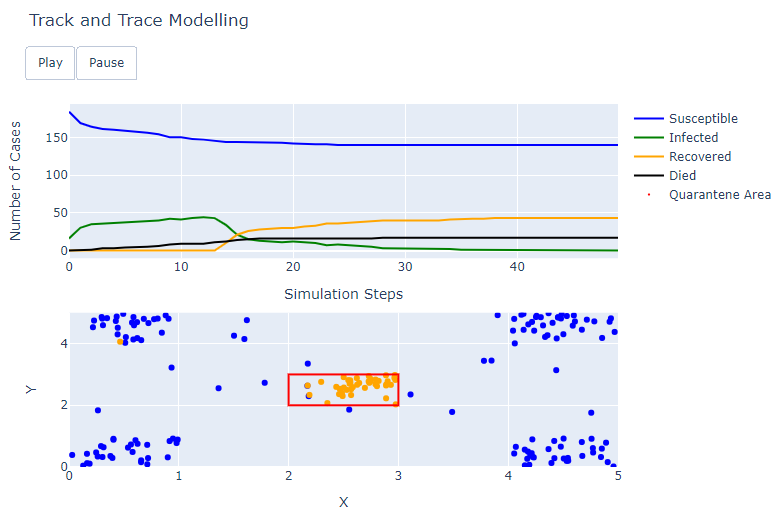
\includegraphics[width=13cm]{latex/images/track1.PNG}%
    \caption{Perfect Track and Tracing}
    \label{track1}
\end{figure}

The following model, extends instead the first model by adding a probability value that some individuals might not get traced at all and might therefore end up spreading the disease (eg. coronavirus asymptomatic or limited available testing capacity). An example simulation result using a 50\% probability to not be traced is shown in Figure \ref{track2}. As the results demonstrated, allowing even a small portion of un-tracked infected individual, can potentially lead to far worse scenarios compared to Figure \ref{track1}. Analogous results have been registered also in \cite{epic}.

\begin{figure}[ht!]%
    \centering
    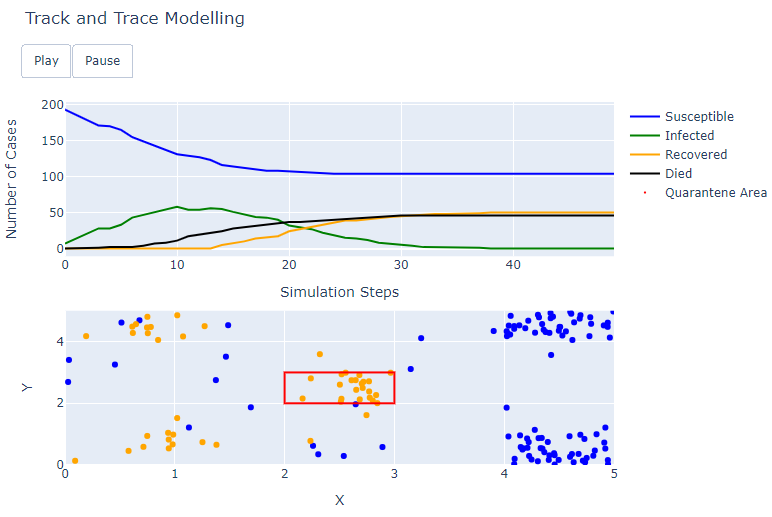
\includegraphics[width=13cm]{latex/images/track2.PNG}%
    \caption{Imperfect Track and Tracing}
    \label{track2}
\end{figure}

\subsection{Central Hubs}

\textbf{Causal Question:} How does having a central hub visited by different communities members effects the spread of the disease?

\textbf{Experimental Results:} Imposing travel restrictions can greatly help in lowering the rate at which a disease can spread. Individuals, although still have at times to visit centrals hubs such as supermarkets during lock-down's. What would be the affect of allowing a central hub on the velocity at which a disease can spread? In this simulation, we can easily observe how having even just a single central hub, can lead to a fast spreading of the disease across different communities.

As the results show in Figure \ref{hub}, allowing about 30\% of the population to visit a central hub, can potentially be quite dangerous because if anyone in the hub is affected, it can then easily allow to spread the disease to individuals belonging to different communities. 

\begin{figure}[ht!]%
    \centering
    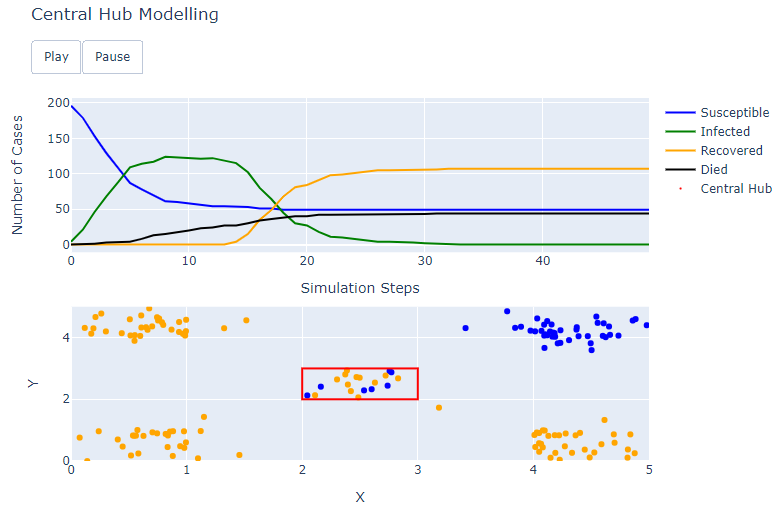
\includegraphics[width=13cm]{latex/images/hubs1.PNG}%
    \caption{Single Central Hub}
    \label{hub}
\end{figure}

\subsection{Finance Simulation}

Applying different types of social distancing and limited movement restrictions, could potentially lead to a good containment of the spreading of a disease, but also to a major shrink of the whole economy. In the following simulation, two main types of responses are simulated: no containment at all or imposing an hard lock-down. In order to keep track of the economic consequences of these two different approaches, the created population has been divided into 3 different classes: Working Class, Middle Class and Upper Class. Which have assigned different types of incomes and expenses which they have to pay on daily bases depending on their income. The government offers the opportunity to give financial support on daily basis in case any of the citizen is struggling to pay its expenses. In a fully functioning society, most of the citizen are able to pay their expenses without having to use their savings or ask for help. As restrictions are imposed and freedom of movement is limited, citizen can only continue to earning and be self-sufficient if they are able to work from home. Otherwise, the will have to make use of their savings and of the government support provided. The financial support covers just the daily expenses and can be asked every day. Because of the nature of their work, middle and higher class workers, are more likely be able to work remotely.

In normal conditions, the updated income of a citizen on daily basis is equal to:

\useshortskip
\begin{align}
\ Updated\:Income = (Income-Expenses)\times \norm{Current\:Position-Previous\:Position}
\label{euc}
\end{align}
\useshortskip

In this way, the ability of moving freely is represented as a way to possibly increase their income (eg. citizen can travel to work and during working activities).

Running an example simulation for 50 days, without applying any restriction, would then lead to the results shown in Figure \ref{fin1}, no financial support requests and overall \textsterling4464.241 of average savings accumulated by the population.

\begin{figure}[ht!]%
    \centering
    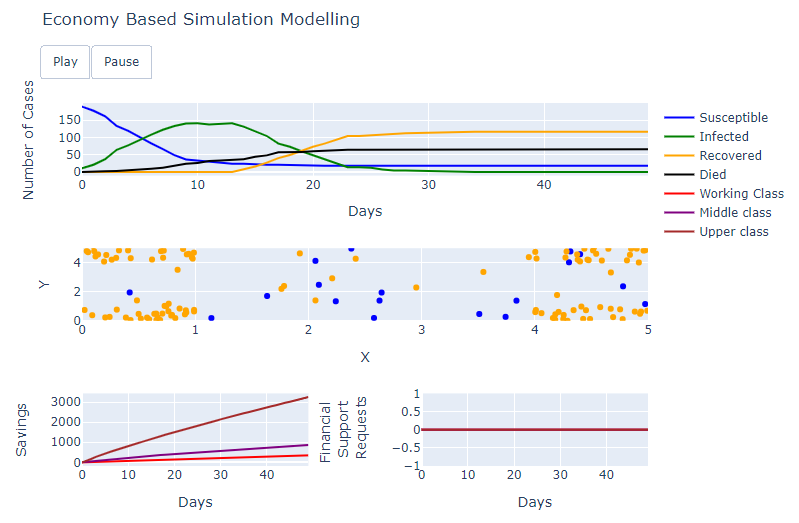
\includegraphics[width=13cm]{latex/images/fin1.PNG}%
    \caption{Financial Modelling (No restrictions applied)}
    \label{fin1}
\end{figure}

Applying instead a lock-down, would then result to just \textsterling3402.764
accumulated savings (mainly from higher social classes) and 241 financial support requests received just from the working class. Applying restrictions, led, on the other side, to a sharp decrease in the overall number of infected and deaths in the community.

\begin{figure}[ht!]%
    \centering
    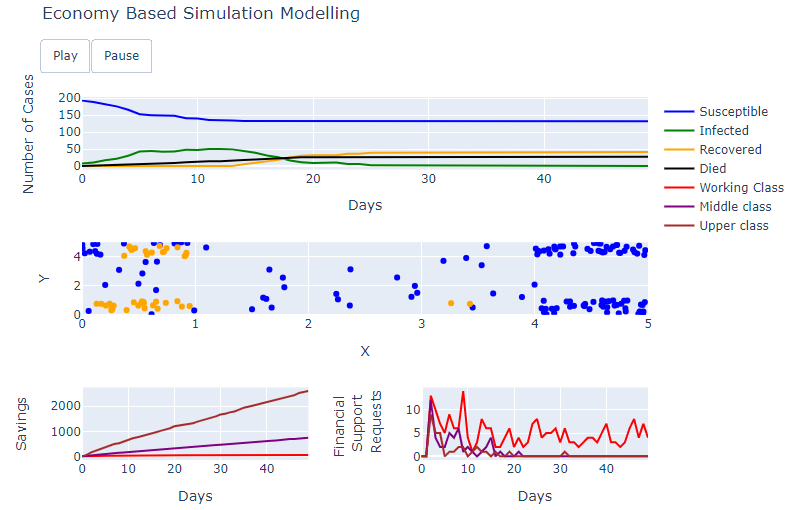
\includegraphics[width=13cm]{latex/images/fin2.PNG}%
    \caption{Financial Modelling (Lock-down)}
    \label{fin2}
\end{figure}

\section{Extras}
In order to make the Web Application, a complete tool which could be used by any type of users, a professional and user-friendly design was created using Streamlit and the app has been made available to the web by creating an Amazon Web Services EC2 Linux Instance. This enabled to easily fetch real time data from various sources and to implement animated an interactive plots.

Some additional features, which have been added to the Web Application are a live report of how Coronavirus has been spreading around the world and live news updates about this topic.

\subsection{Live World Statistics and Records}

In this section of the Web Application, summary statistics of the number of cases/recovered/deaths due to Coronavirus, have been provided (Figure \ref{world}). 

\begin{figure}[ht!]%
    \centering
    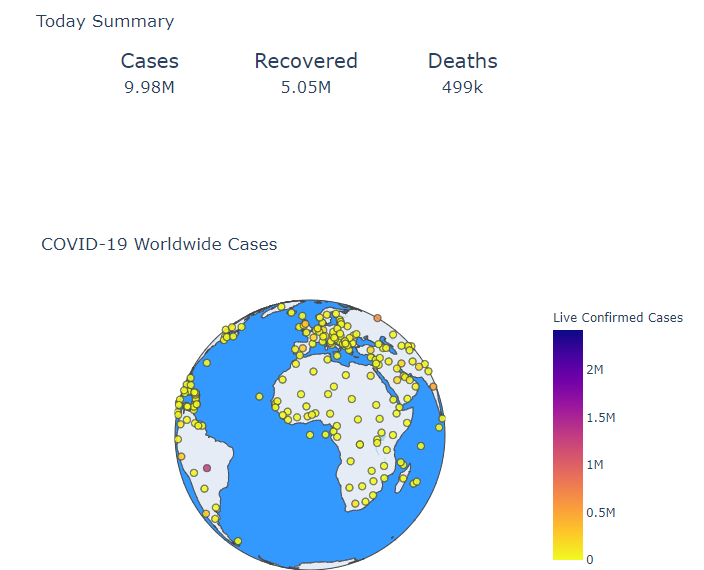
\includegraphics[width=11cm]{latex/images/world.PNG}%
    \caption{World Statistics Example}
    \label{world}
\end{figure}

These included:

\begin{itemize}
    \setlength\itemsep{-0.3cm}
    \item Record of the number of cases/recovered/deaths in the world up to date.
    \item Interactive world view of how the number of cases are spread around the word.
    \item Charts displaying what are today's top 10 countries for number of cases and deaths and how their numbers changed in the last 24 hours.
    \item Interactive animations displaying how Coronavirus spread across different countries over time.
\end{itemize}

The data used in order to create these charts, was provided by the Center for Systems Science and Engineering (CSSE) at Johns Hopkins University \cite{world_data} and automatically updated every 24hrs.

\subsection{Live World News and Sentiment Analysis}

This section was possible thanks to the use of the Python News API \cite{news}, making use of this API are in fact fetched every 2 hours news from a large number of countries around the world about Coronavirus. 

\begin{figure}[ht!]%
    \centering
    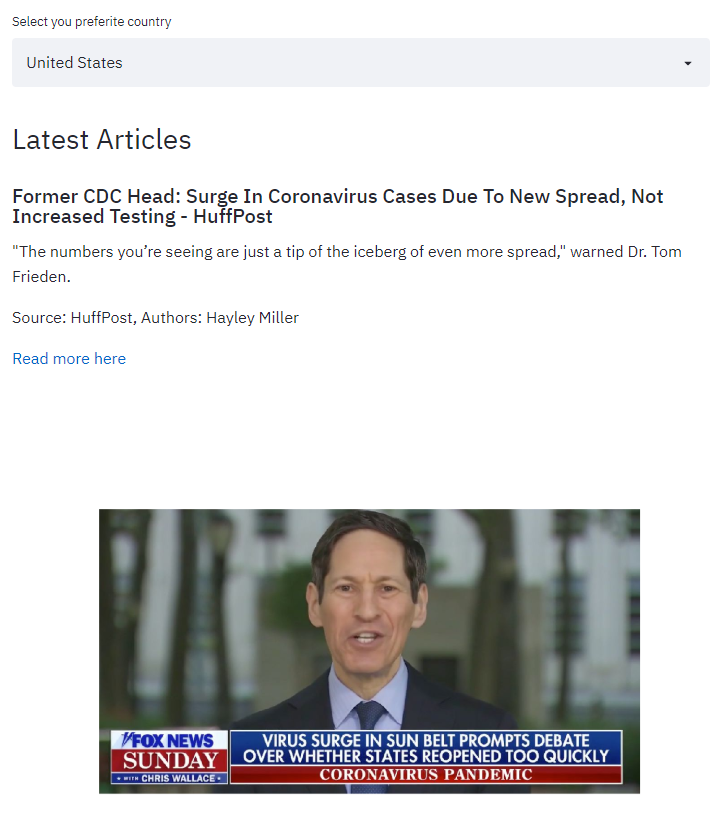
\includegraphics[width=9cm]{latex/images/news.PNG}%
    \caption{World News Example}
    \label{news}
\end{figure}

Using the fetched news article, it was then possible to apply sentiment analysis in each of the different countries in order to understand what are the key words of the day and what's the overall sentiment about the outbreak. Standard Natural Language Pre-processing techniques (eg. Tokenizzation, Stop Words Removal, Stemming) have been applied using the Python NLTK (Natural Language Toolkit) library and the sentiment was calculated using the VADER (Valence Aware Dictionary and sEntiment Reasoner) model. This type of model would then return a sentiment score between -1 (negative) and 1 (positive).

\begin{figure}[ht!]%
    \centering
    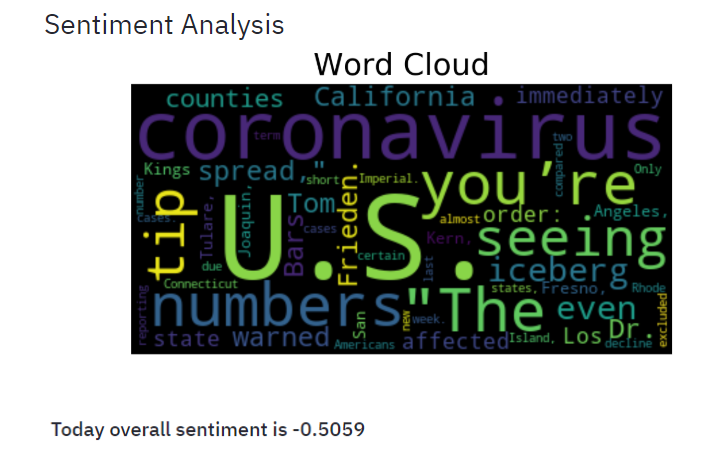
\includegraphics[width=10cm]{latex/images/news2.PNG}%
    \caption{World News Sentiment Analysis}
    \label{news2}
\end{figure}
